\begin{figure}[!h]
    \centering
    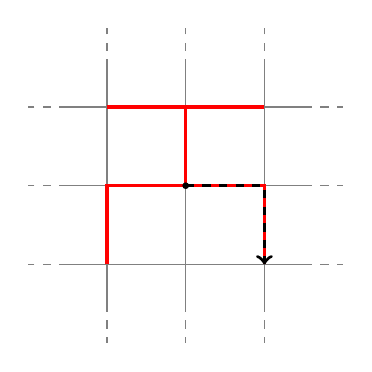
\begin{tikzpicture}
        \foreach \i in {-1, 0, 1} {
            \draw[gray] (-1.5, \i) -- (1.5, \i);
            \draw[gray] (\i, -1.5) -- (\i, 1.5);
            
            \draw[gray, dashed] (-1.5, \i) -- (-2.0, \i);
            \draw[gray, dashed] (\i, -1.5) -- (\i, -2.0);
            \draw[gray, dashed] (1.5, \i) -- (2.0, \i);
            \draw[gray, dashed] (\i, 1.5) -- (\i, 2.0);
        }
        
        \draw[red, very thick] (0, 0) -- (0, 1);
        \draw[red, very thick] (-1, 1) -- (1, 1);
        \draw[red, very thick] (-1, -1) -- (-1, 0) -- (0, 0);
        
        \draw[red, very thick] (0, 0) -- (1, 0) -- (1, -1);
        \draw[->, dashed, very thick] (0, 0) -- (1, 0) -- (1, -1);
        
        \filldraw (0, 0) circle (1pt);
        
    \end{tikzpicture}
    \caption{A self-avoiding path of length $2$ from $O$: the event $\abs{C} \geq 3$ occurs.}
    \label{fig:cluster_self_avoiding_path}
\end{figure}